\chapter{Validation de la simulation des variables de forme de gerbes �lectromagn�tiques avec des muons cosmiques}

\begin{figure}[!ht]
  \begin{center}

  \begin{tabular}{cc}
    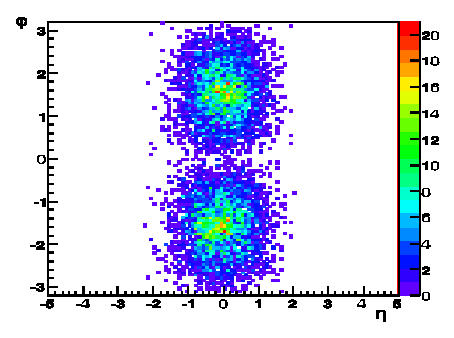
\includegraphics[height=5.25cm, keepaspectratio]{phd_cosmics/cmp1a}
    &
    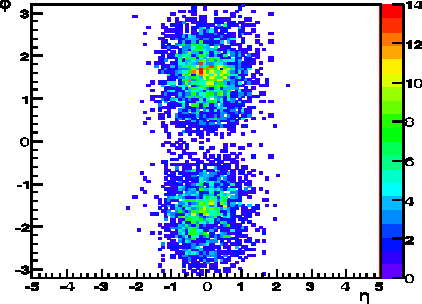
\includegraphics[height=5.25cm, keepaspectratio]{phd_cosmics/cmp1b}
    \\
    (a) & (b)
  \end{tabular}

  \end{center}
  \caption{}
\end{figure}

\begin{figure}[!ht]
  \begin{center}

  \begin{tabular}{cc}
    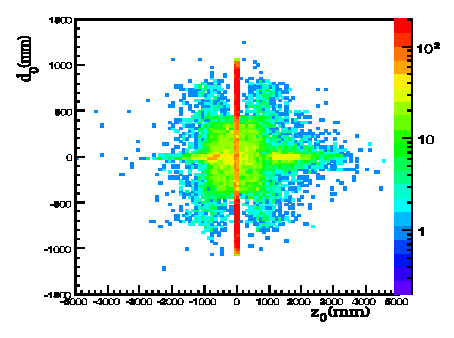
\includegraphics[height=5.25cm, keepaspectratio]{phd_cosmics/cmp2a}
    &
    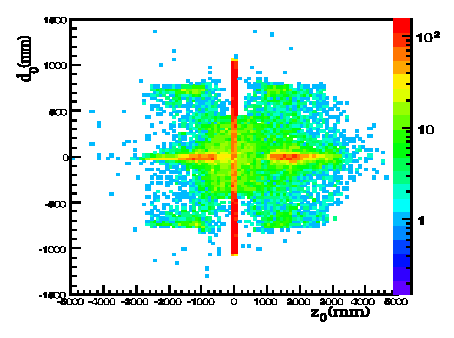
\includegraphics[height=5.25cm, keepaspectratio]{phd_cosmics/cmp2b}
    \\
    (a) & (b)
  \end{tabular}

  \end{center}
  \caption{}
\end{figure}

\begin{figure}[!ht]
  \begin{center}

  \begin{tabular}{cc}
    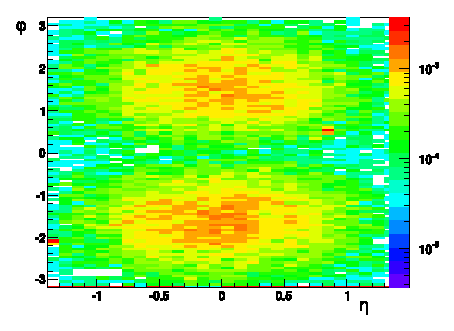
\includegraphics[height=5.25cm, keepaspectratio]{phd_cosmics/cmp3a}
    &
    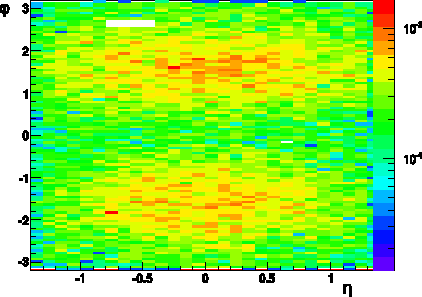
\includegraphics[height=5.25cm, keepaspectratio]{phd_cosmics/cmp3b}
    \\
    (a) & (b)
  \end{tabular}

  \end{center}
  \caption{}
\end{figure}

\begin{figure}[!ht]
  \begin{center}

  \begin{tabular}{cc}
    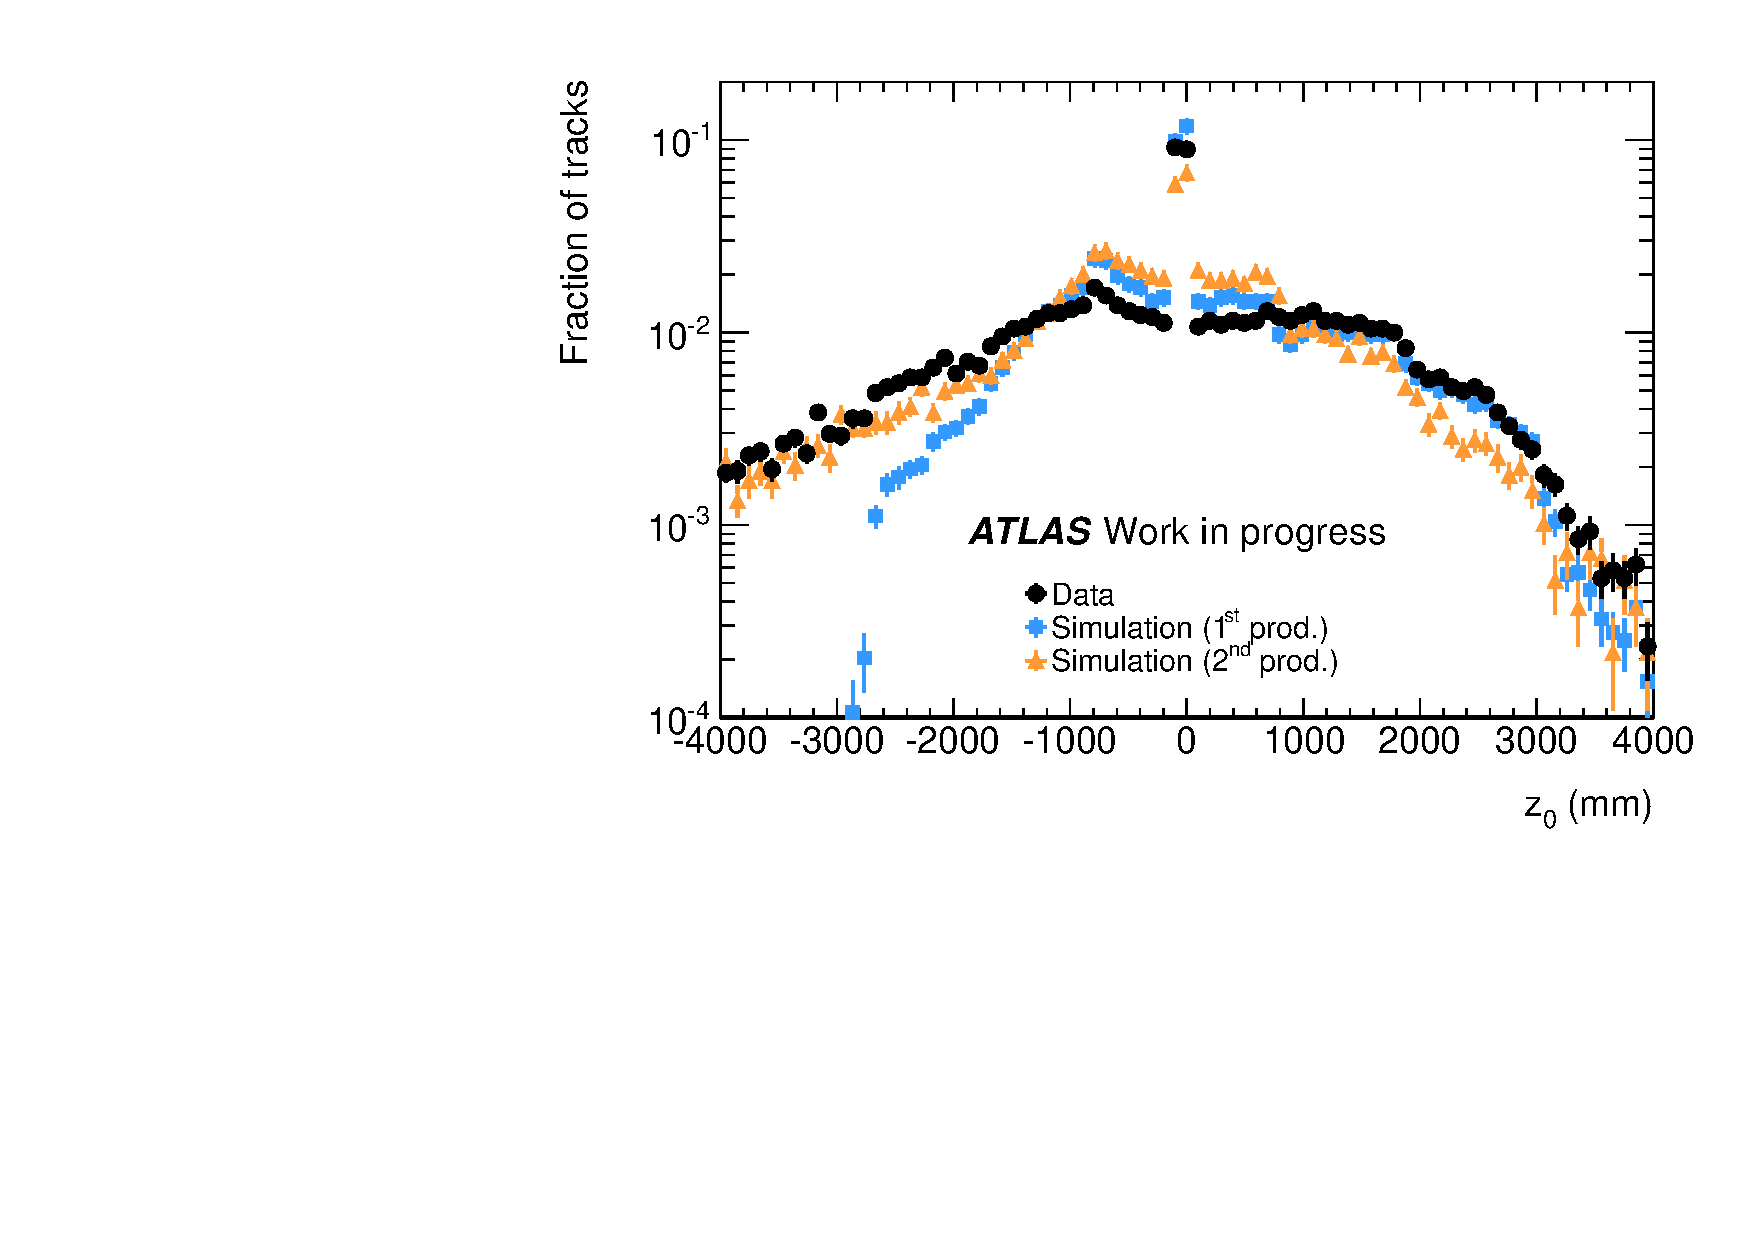
\includegraphics[height=5.25cm, keepaspectratio]{phd_cosmics/z0}
    &
    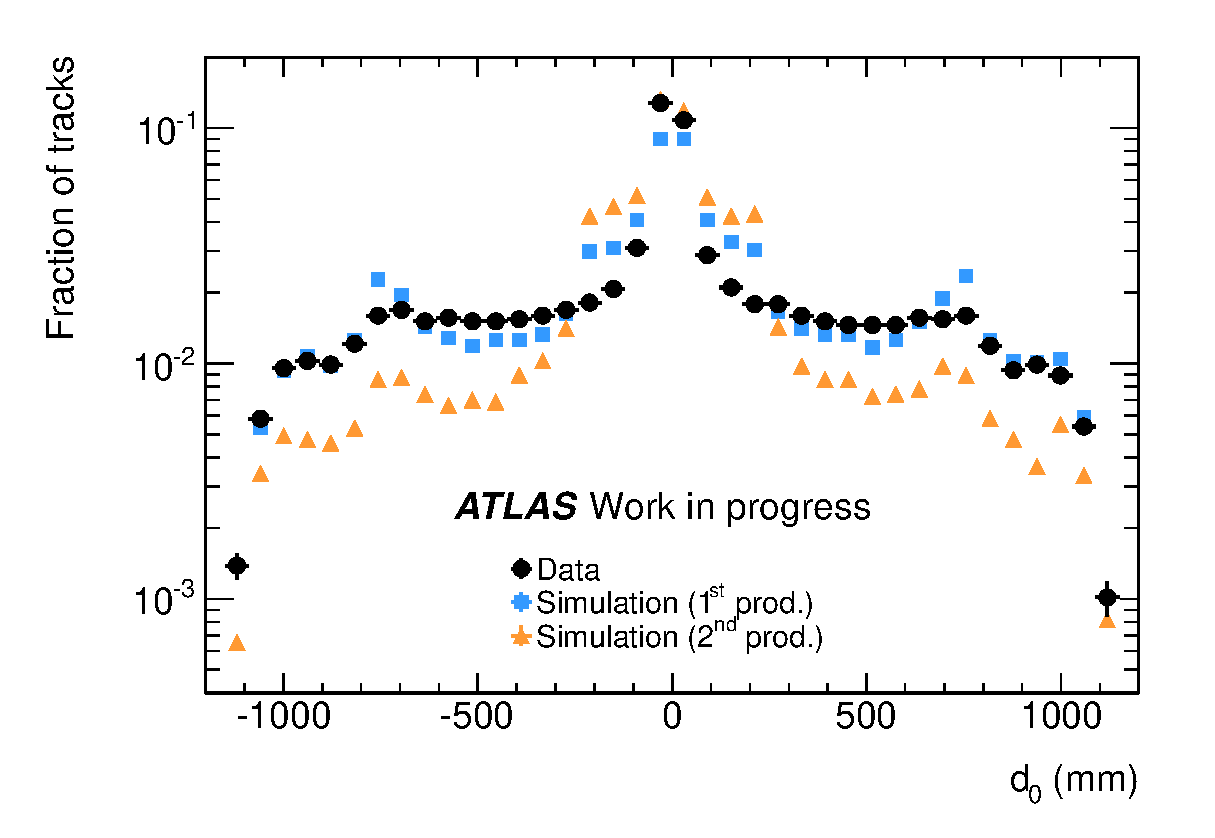
\includegraphics[height=5.25cm, keepaspectratio]{phd_cosmics/d0}
    \\
    (a) & (b)
  \end{tabular}

  \end{center}
  \caption{}
\end{figure}

\begin{figure}[!ht]
  \begin{center}

  \begin{tabular}{ccc}
    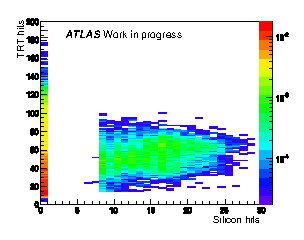
\includegraphics[height=3.75cm, keepaspectratio]{phd_cosmics/hits1}
    &
    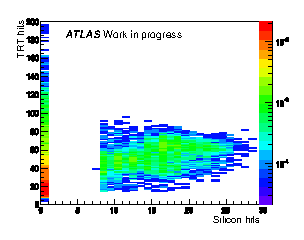
\includegraphics[height=3.75cm, keepaspectratio]{phd_cosmics/hits2}
    &
    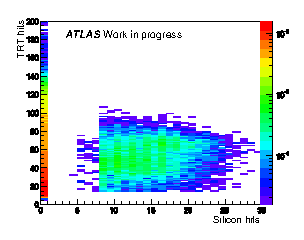
\includegraphics[height=3.75cm, keepaspectratio]{phd_cosmics/hits3}
    \\
    (a) & (b) & (c)
  \end{tabular}

  \end{center}
  \caption{}
\end{figure}

\begin{figure}[!ht]
  \begin{center}

  \begin{tabular}{ccc}
    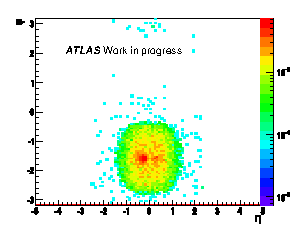
\includegraphics[height=3.75cm, keepaspectratio]{phd_cosmics/cl1}
    &
    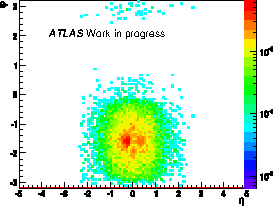
\includegraphics[height=3.75cm, keepaspectratio]{phd_cosmics/cl2}
    &
    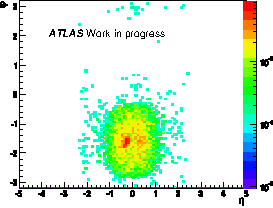
\includegraphics[height=3.75cm, keepaspectratio]{phd_cosmics/cl3}
    \\
    (a) & (b) & (c)
  \end{tabular}

  \end{center}
  \caption{}
\end{figure}

\begin{figure}[!ht]
  \begin{center}

  \begin{tabular}{ccc}
    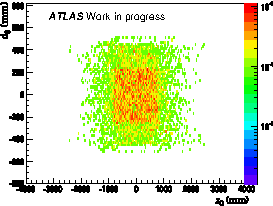
\includegraphics[height=3.75cm, keepaspectratio]{phd_cosmics/trk1}
    &
    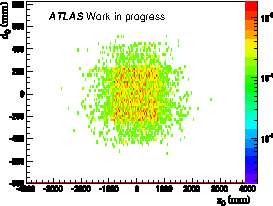
\includegraphics[height=3.75cm, keepaspectratio]{phd_cosmics/trk2}
    &
    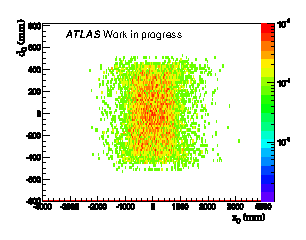
\includegraphics[height=3.75cm, keepaspectratio]{phd_cosmics/trk3}
    \\
    (a) & (b) & (c)
  \end{tabular}

  \end{center}
  \caption{}
\end{figure}

\begin{figure}[!ht]
  \begin{center}

  \begin{tabular}{cc}
    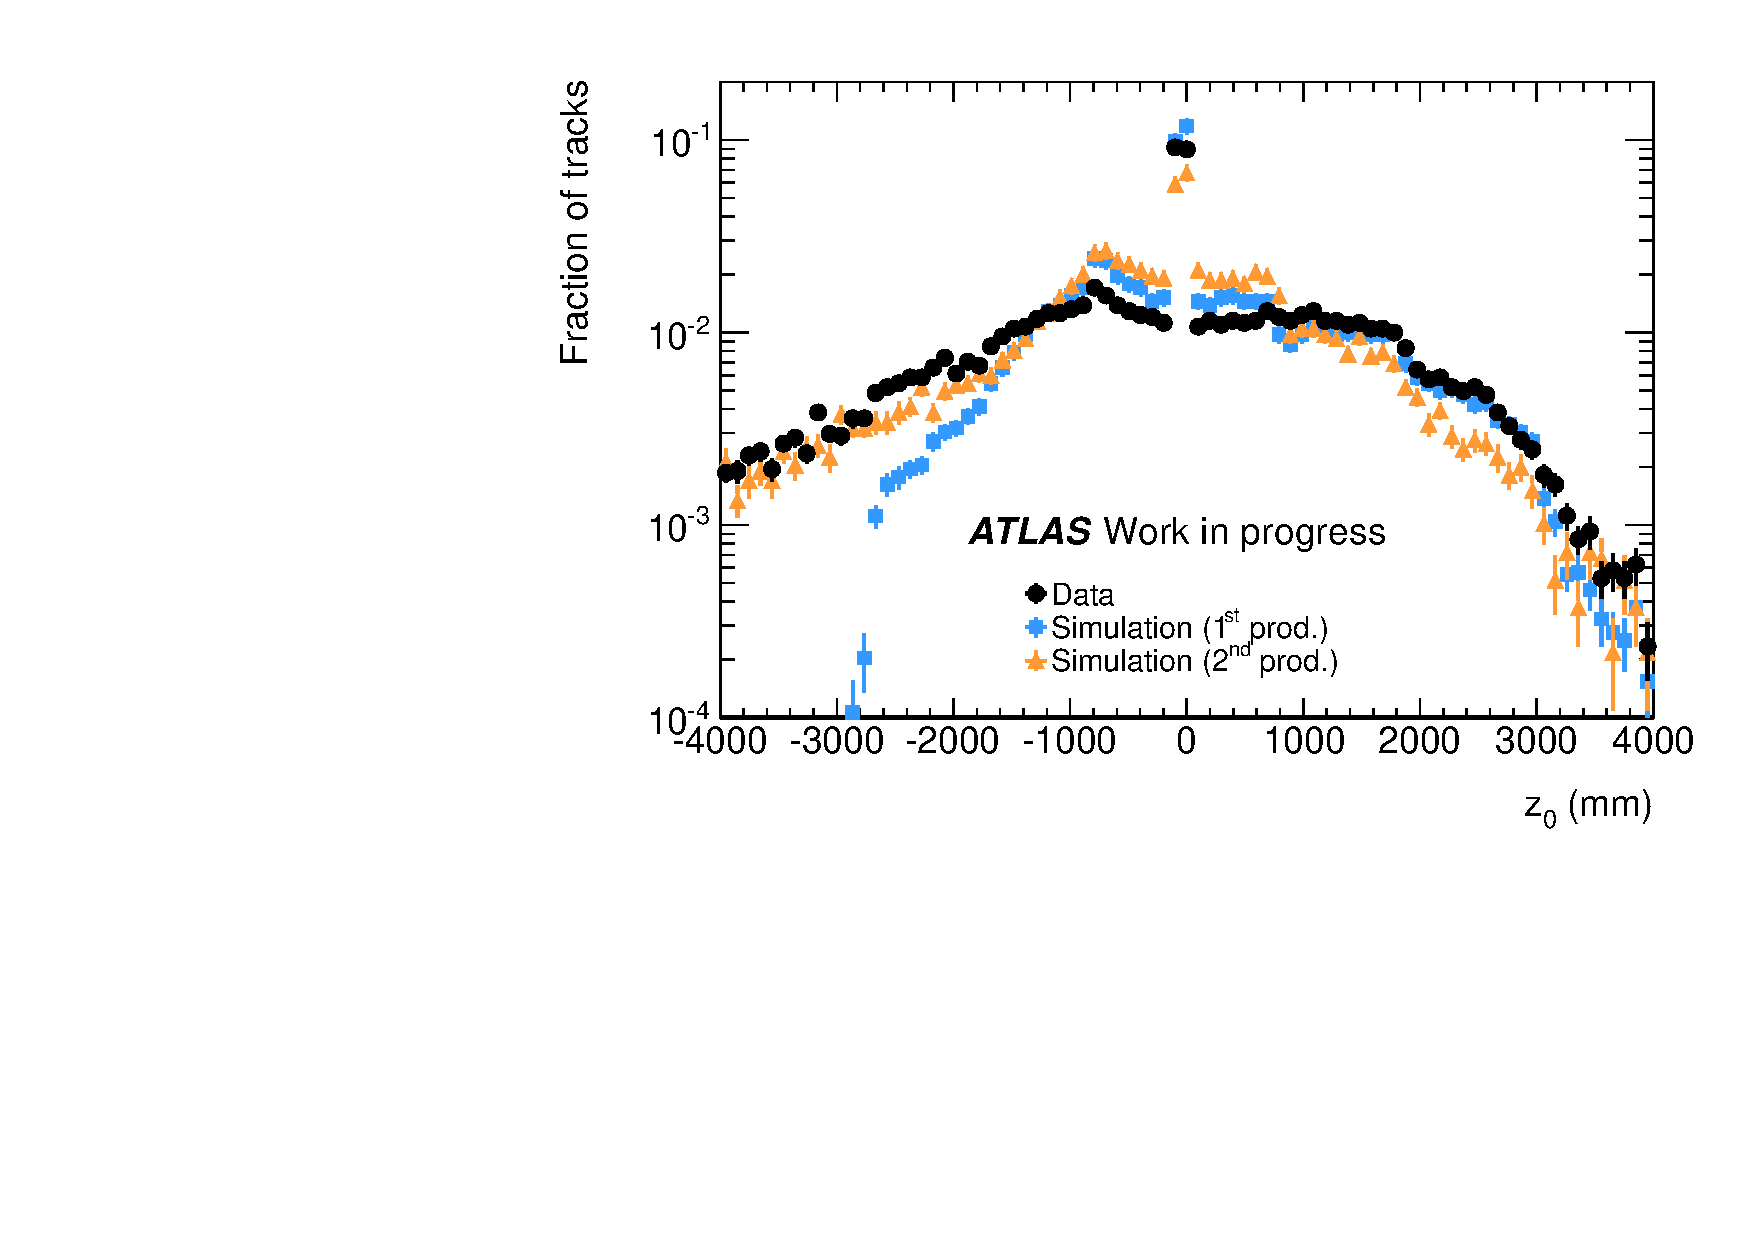
\includegraphics[height=5.25cm, keepaspectratio]{phd_cosmics/z0}
    &
    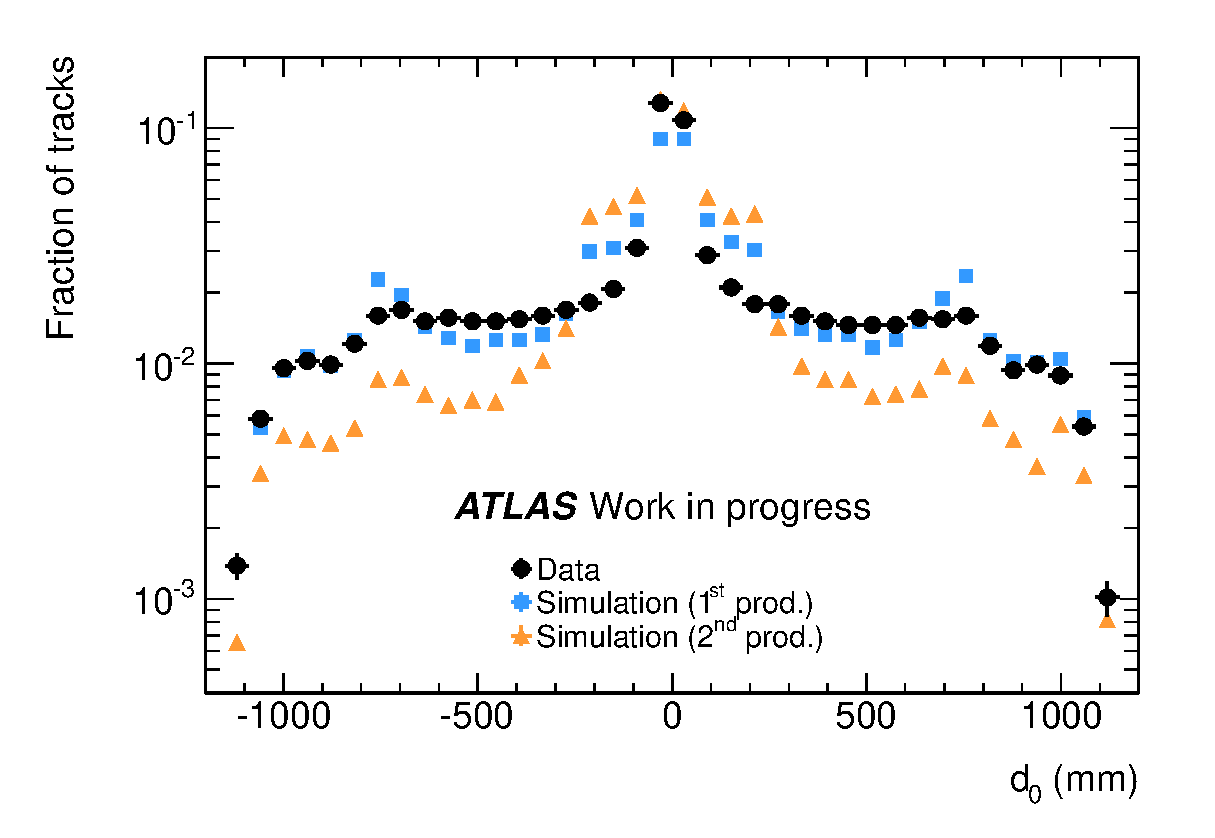
\includegraphics[height=5.25cm, keepaspectratio]{phd_cosmics/d0}
    \\
    (a) & (b)
    \\
    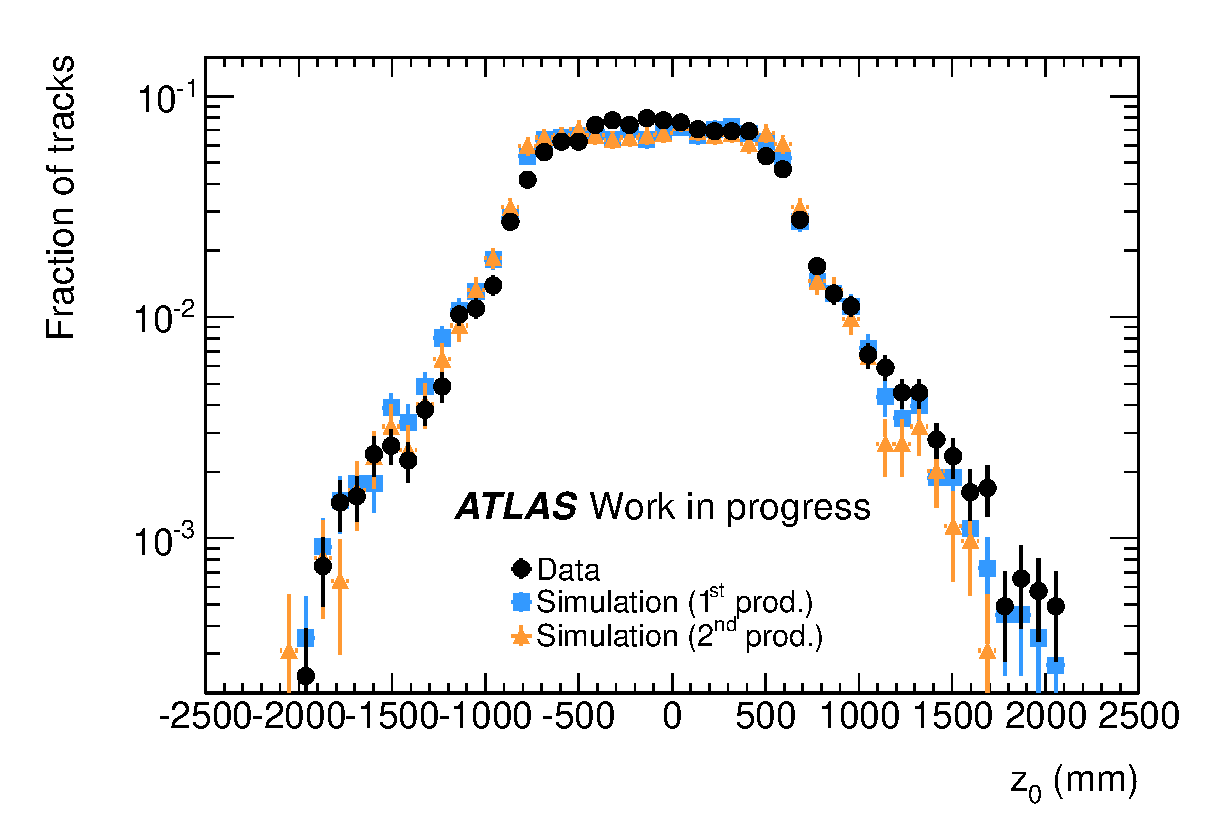
\includegraphics[height=5.25cm, keepaspectratio]{phd_cosmics/z0selected}
    &
    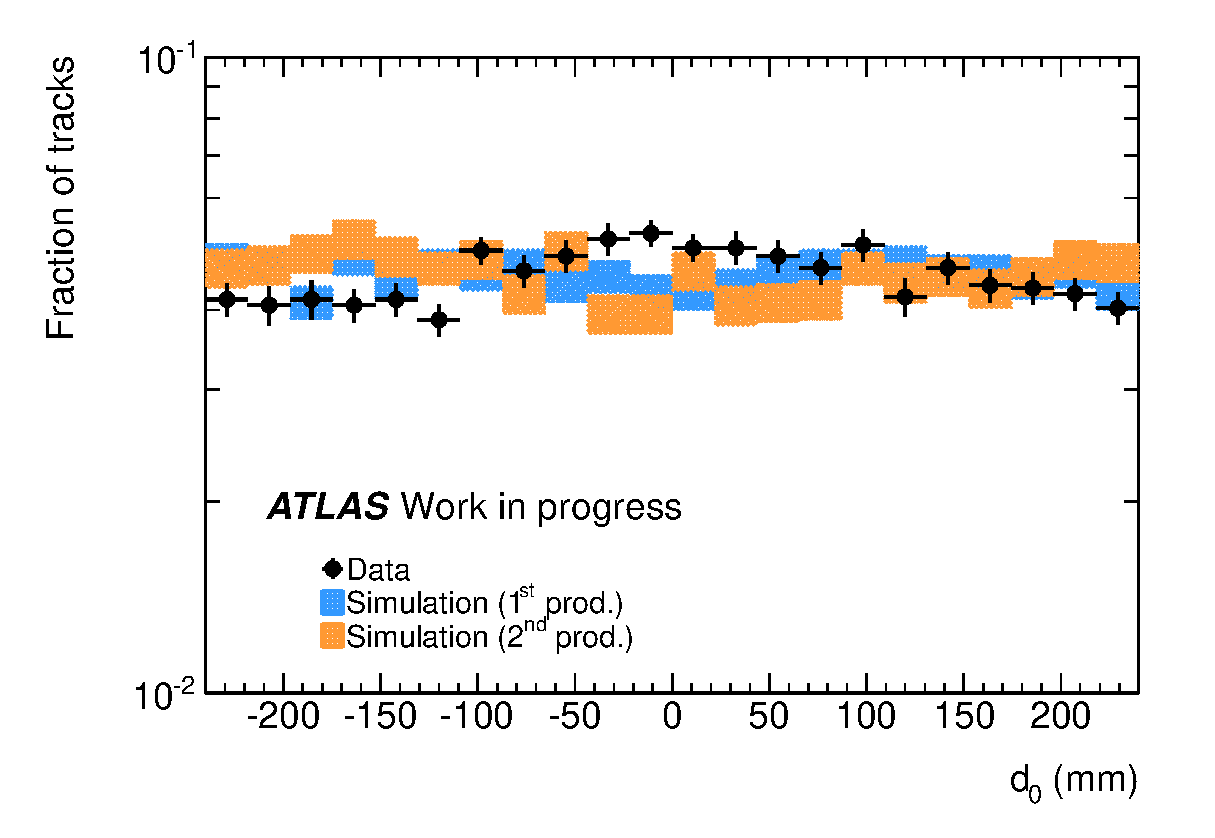
\includegraphics[height=5.25cm, keepaspectratio]{phd_cosmics/d0selected}
    \\
    (c) & (d)
  \end{tabular}

  \end{center}
  \caption{}
\end{figure}

\begin{figure}[!ht]
  \begin{center}
    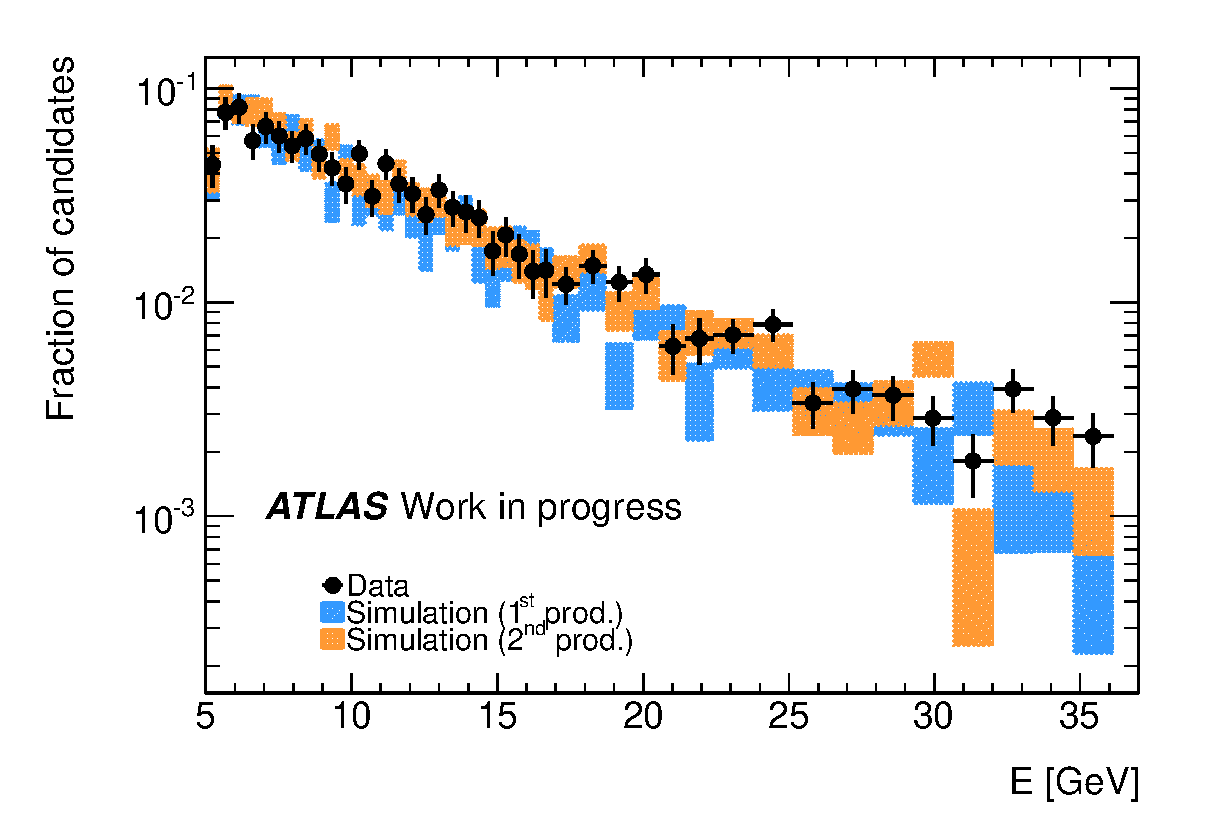
\includegraphics[height=5.25cm, keepaspectratio]{phd_cosmics/spectrum}
  \end{center}
  \caption{}
\end{figure}

\begin{figure}[!ht]
  \begin{center}
    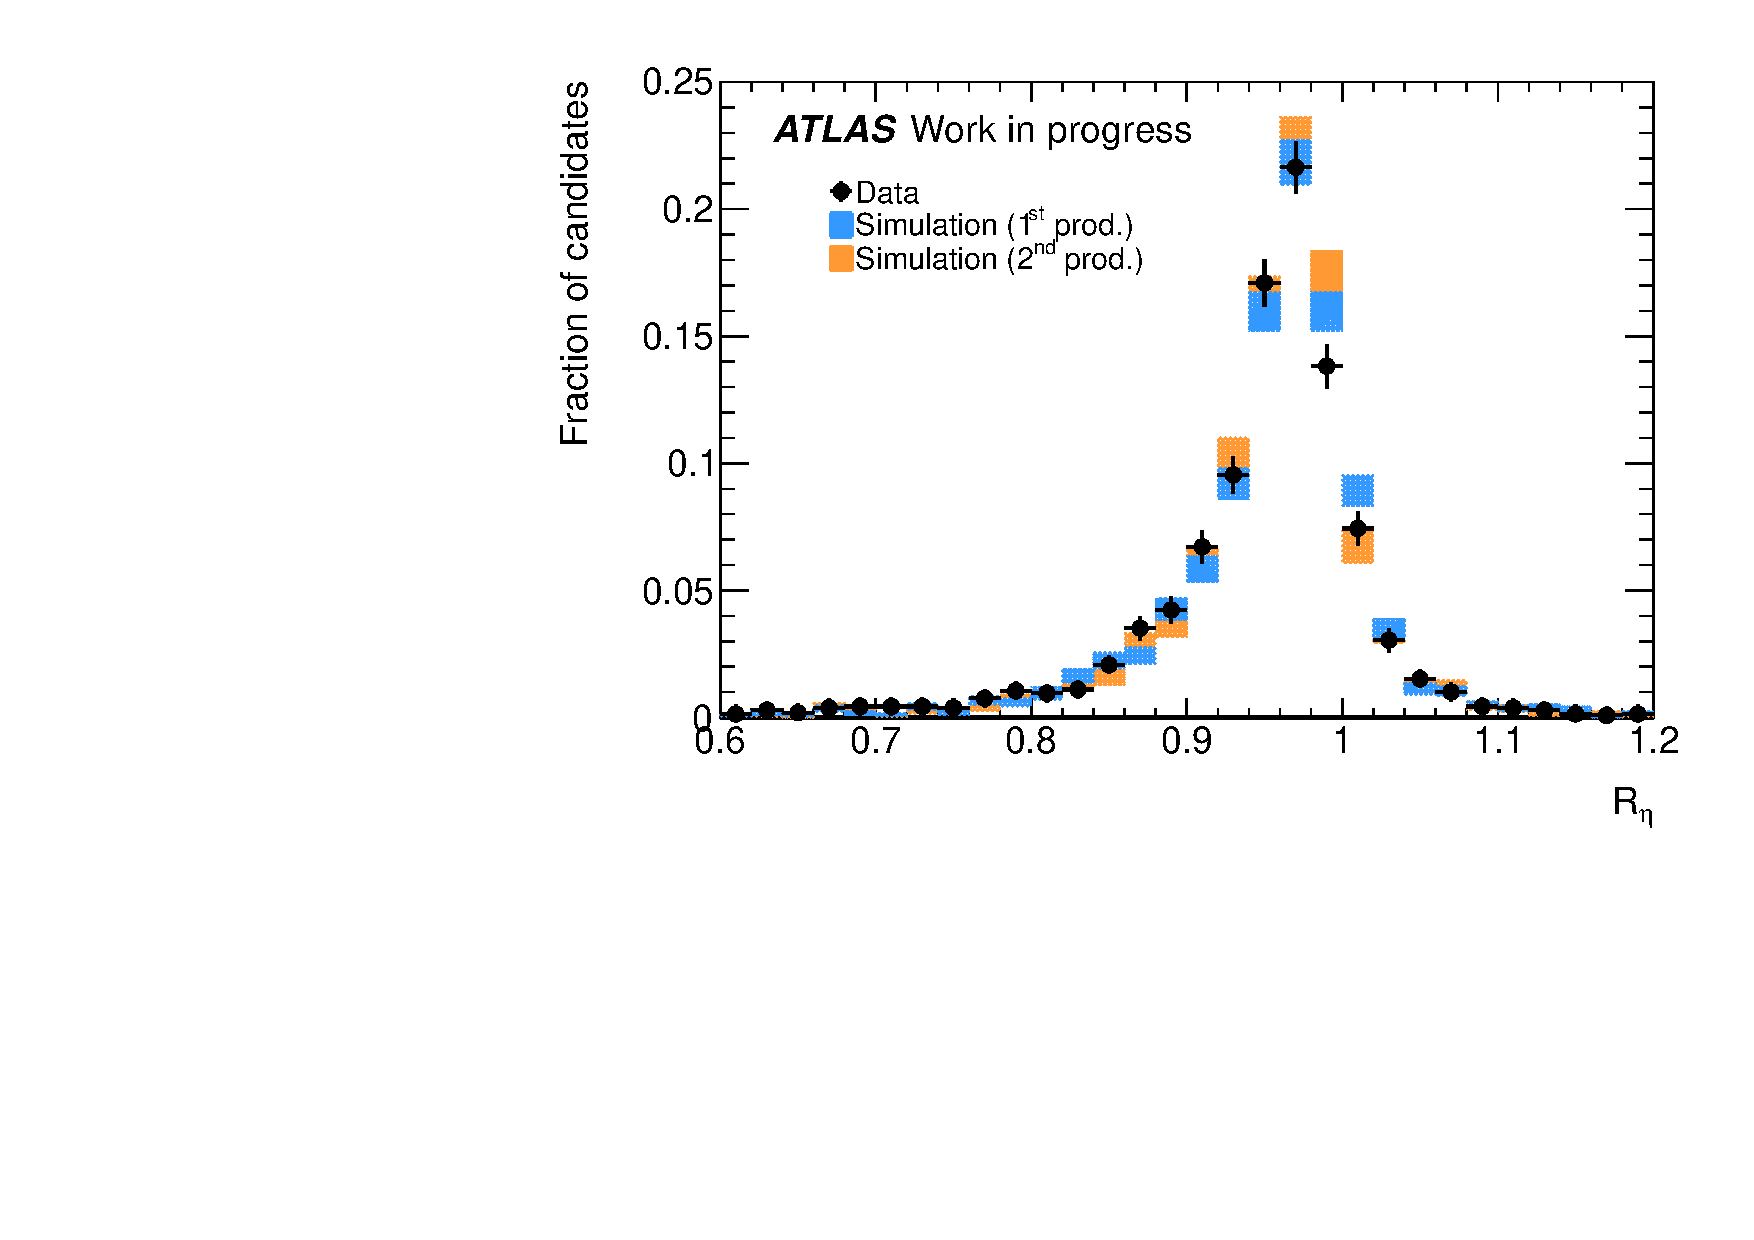
\includegraphics[height=5.25cm, keepaspectratio]{phd_cosmics/reta}
  \end{center}
  \caption{}
\end{figure}

\begin{figure}[!ht]
  \begin{center}

  \begin{tabular}{cc}
    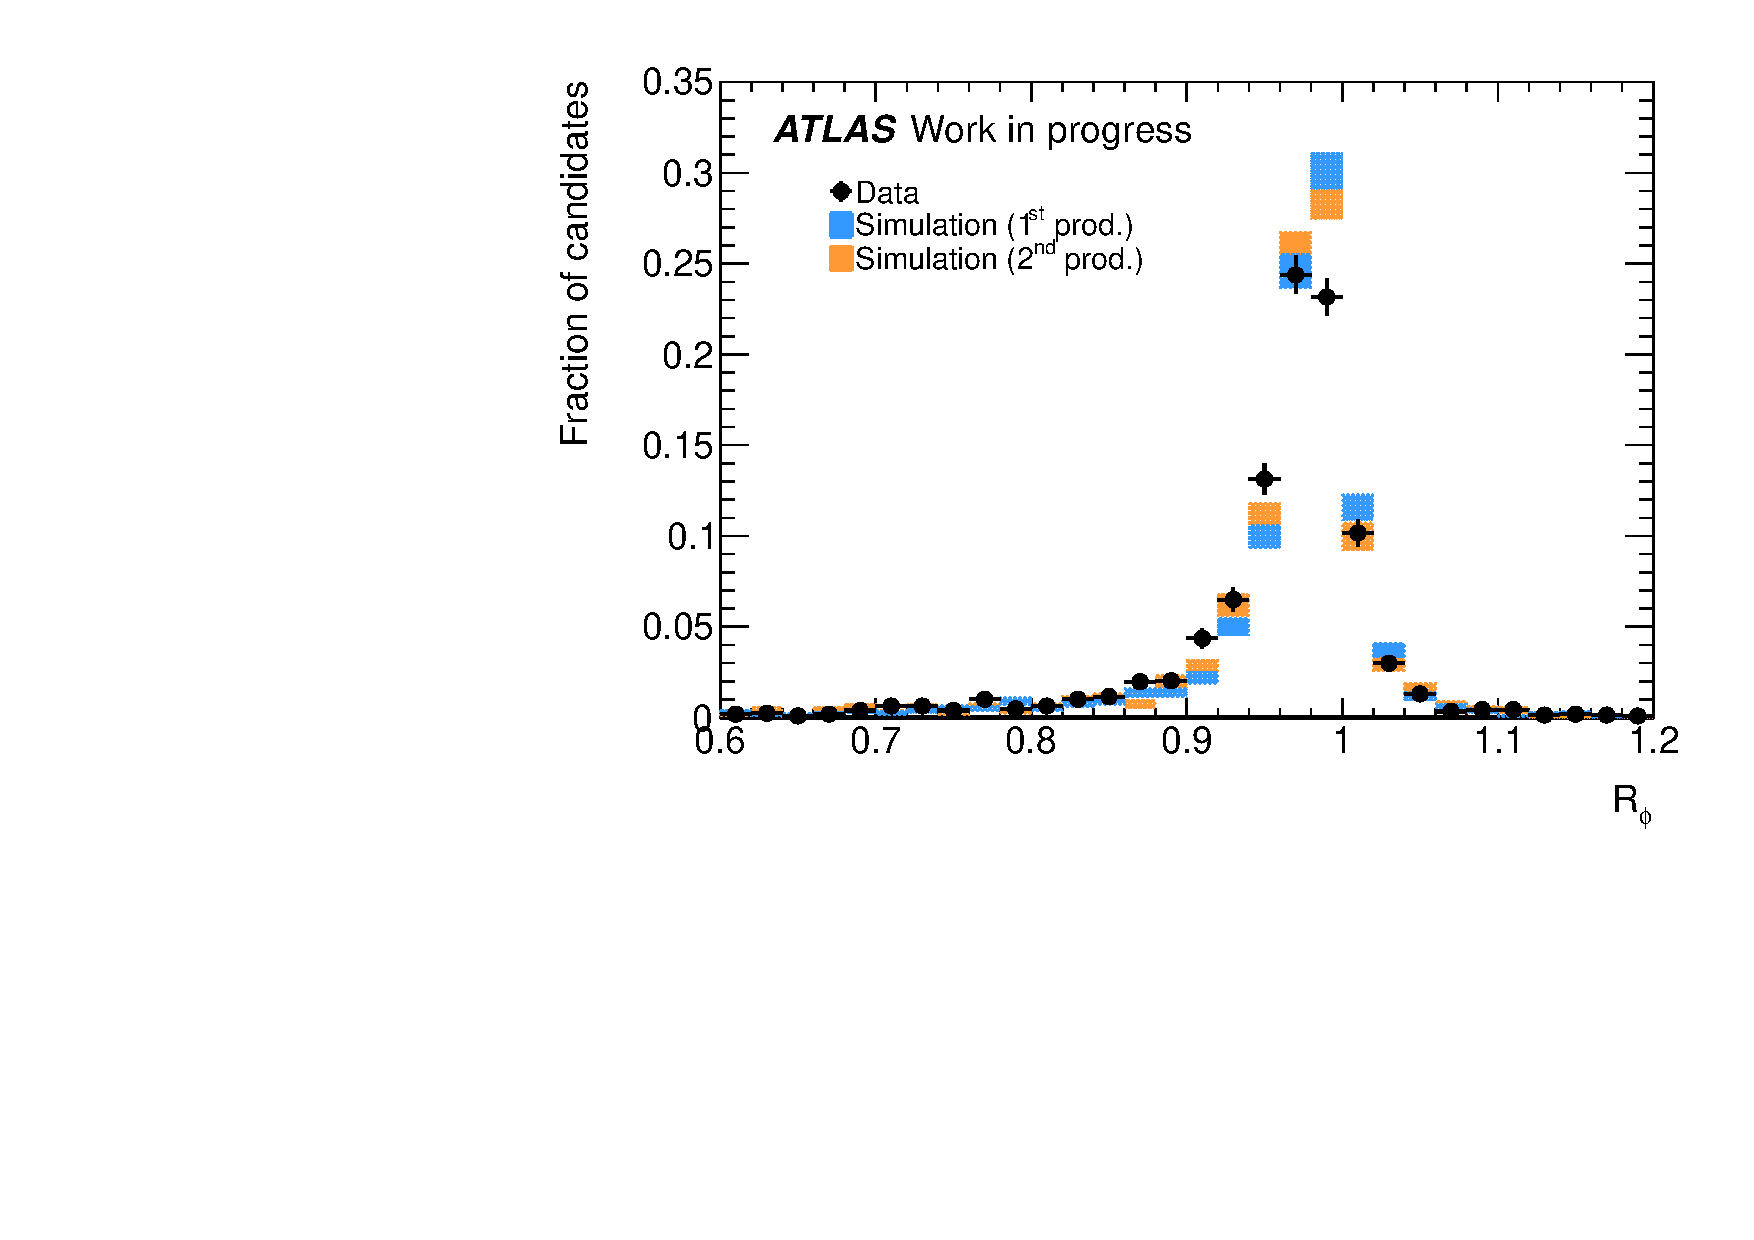
\includegraphics[height=5.25cm, keepaspectratio]{phd_cosmics/rphi}
    &
    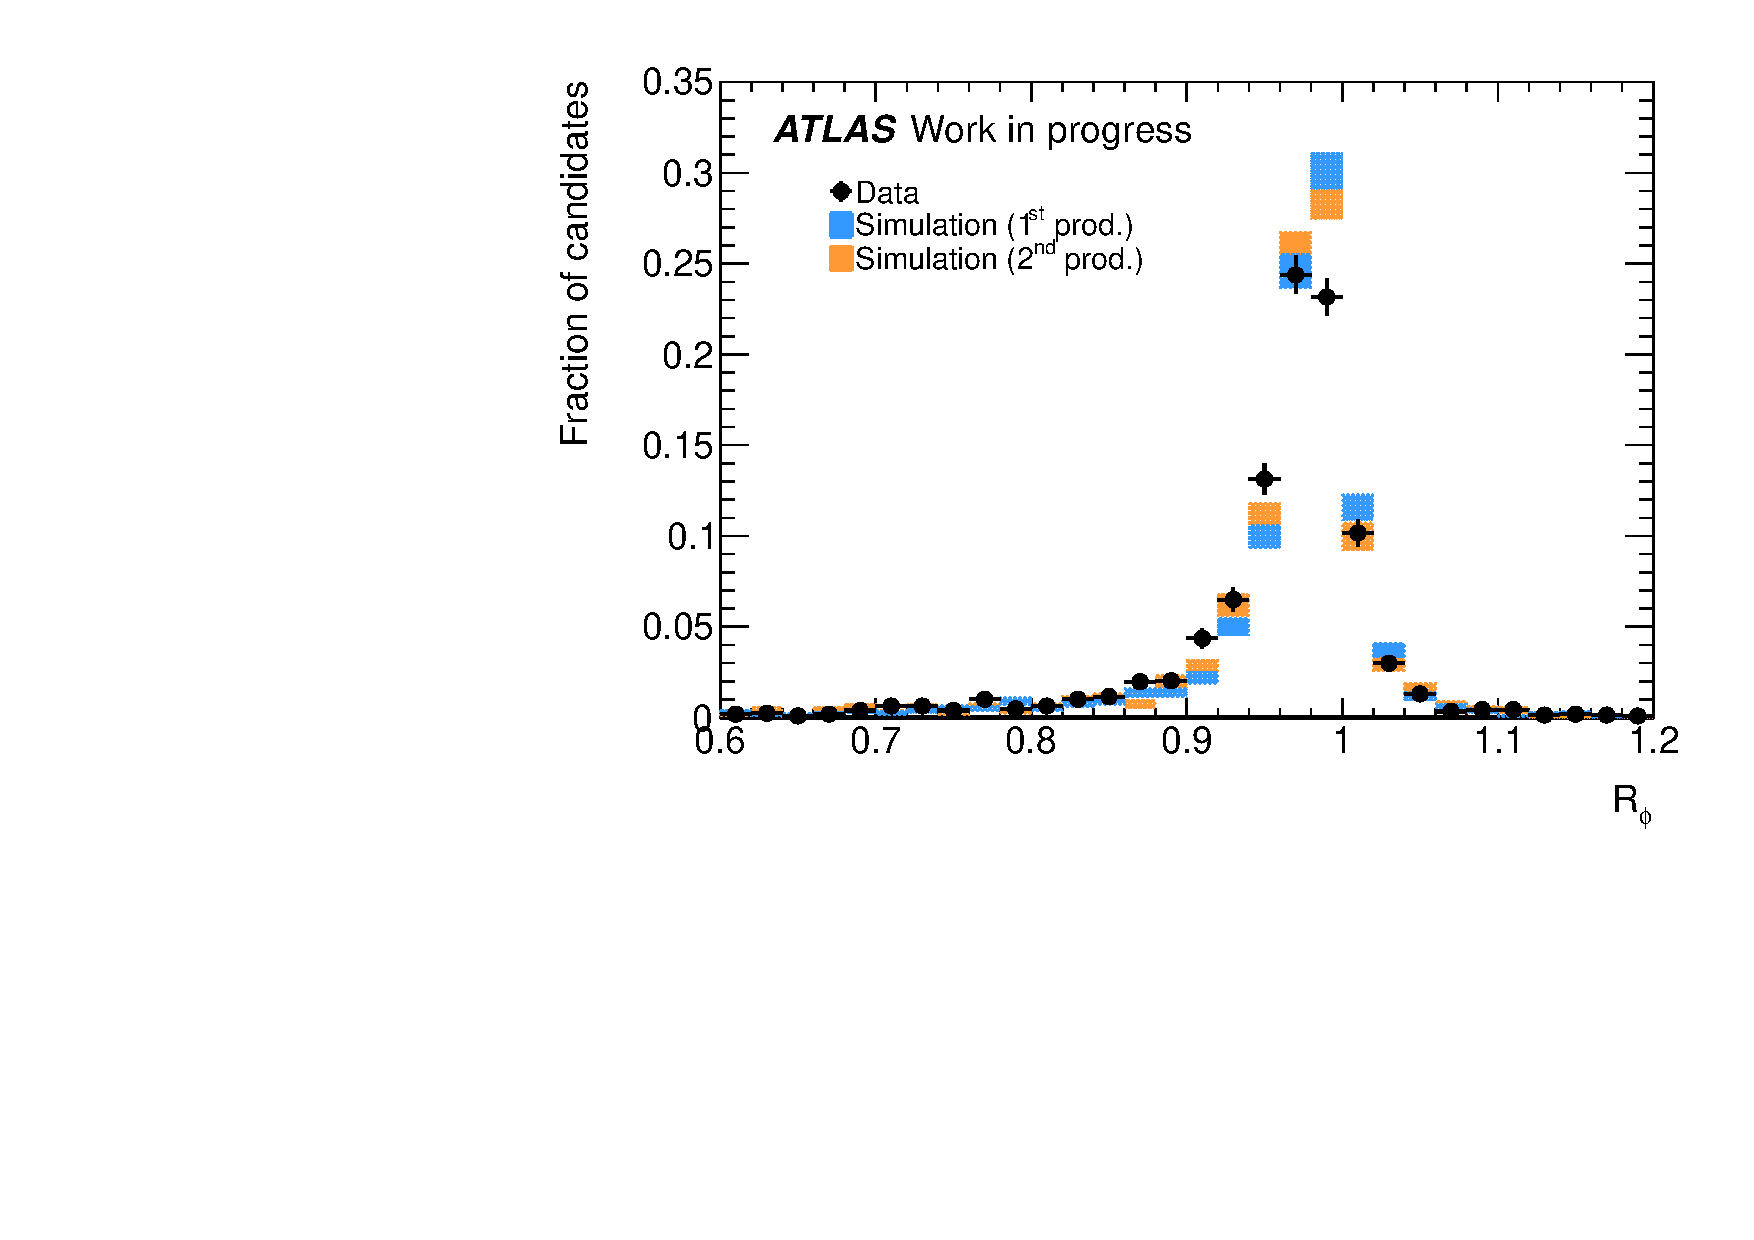
\includegraphics[height=5.25cm, keepaspectratio]{phd_cosmics/rphi}
    \\
    (a) & (b)
  \end{tabular}

  \end{center}
  \caption{}
\end{figure}

\begin{figure}[!ht]
  \begin{center}
    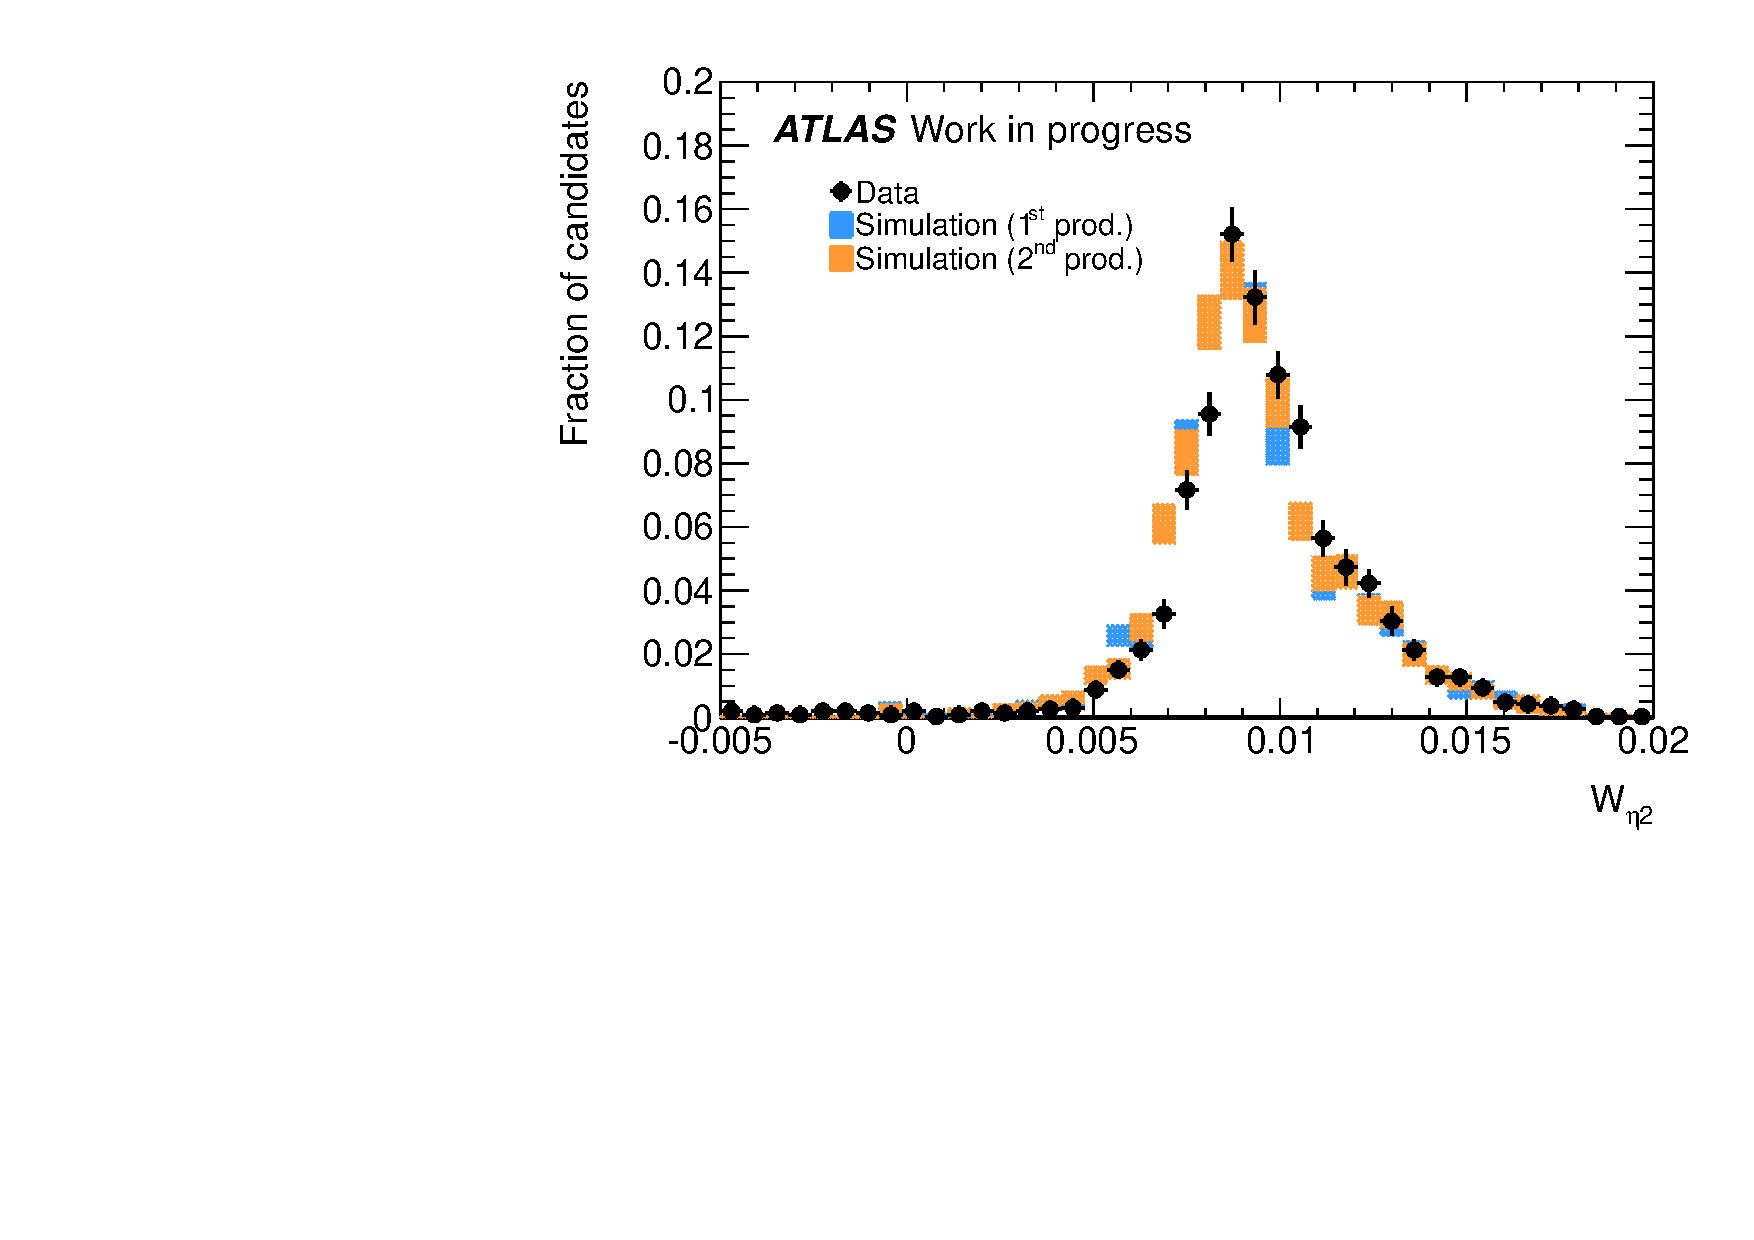
\includegraphics[height=5.25cm, keepaspectratio]{phd_cosmics/weta2}
  \end{center}
  \caption{}
\end{figure}

\begin{figure}[!ht]
  \begin{center}

  \begin{tabular}{ccc}
    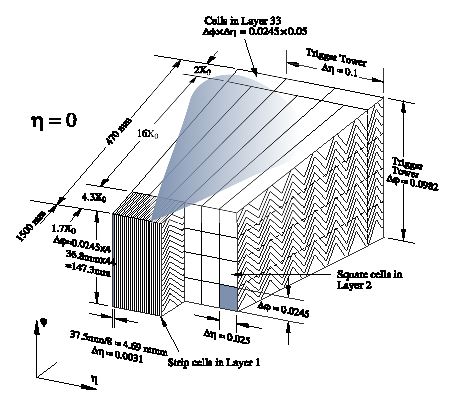
\includegraphics[height=6.75cm, keepaspectratio]{phd_cosmics/caloa}
    &&
    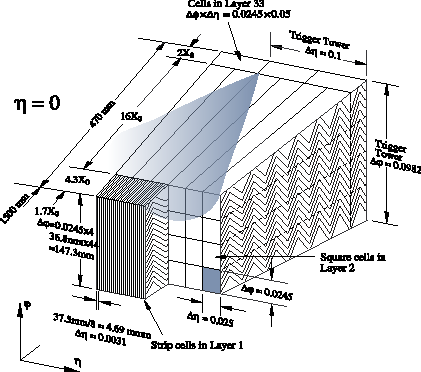
\includegraphics[height=6.75cm, keepaspectratio]{phd_cosmics/calob}
    \\
    (a) && (b)
  \end{tabular}

  \end{center}
  \caption{}
\end{figure}

\begin{figure}[!ht]
  \begin{center}

  \begin{tabular}{cc}
    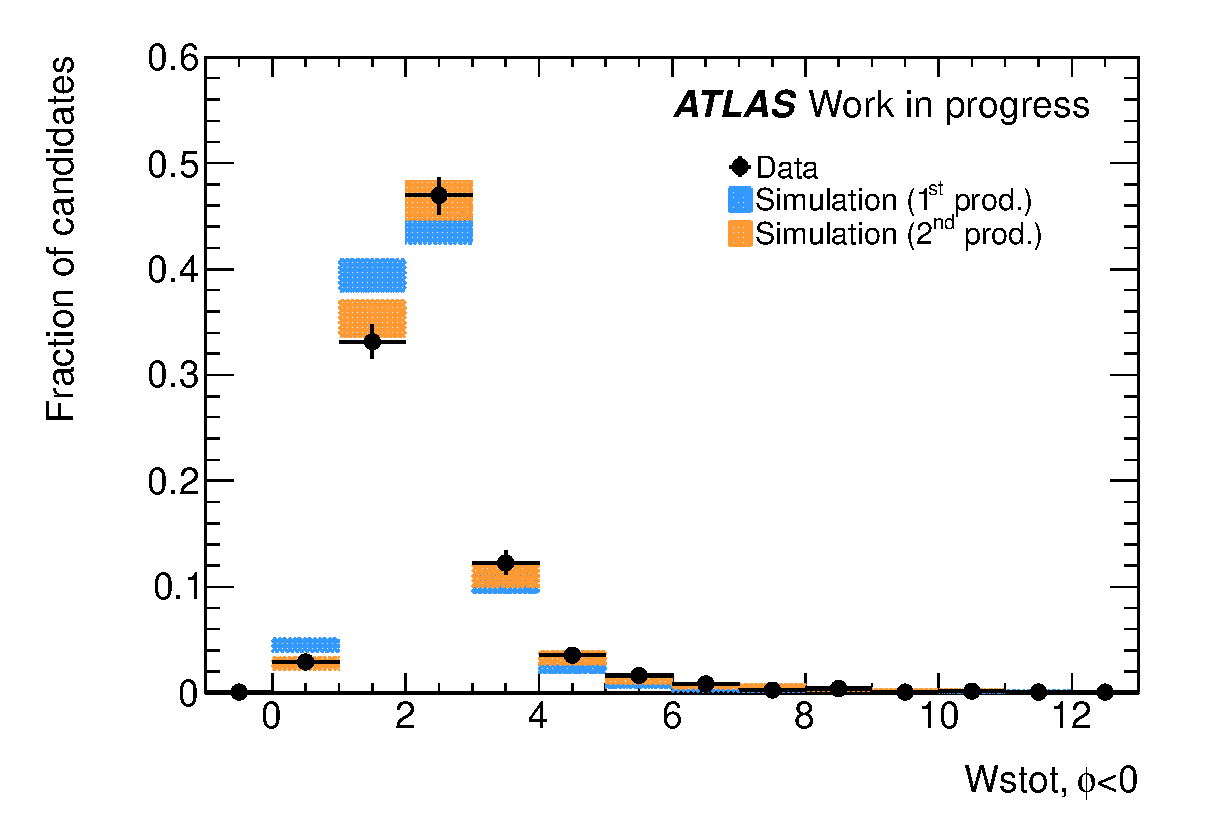
\includegraphics[height=5.25cm, keepaspectratio]{phd_cosmics/wstotDw}
    &
    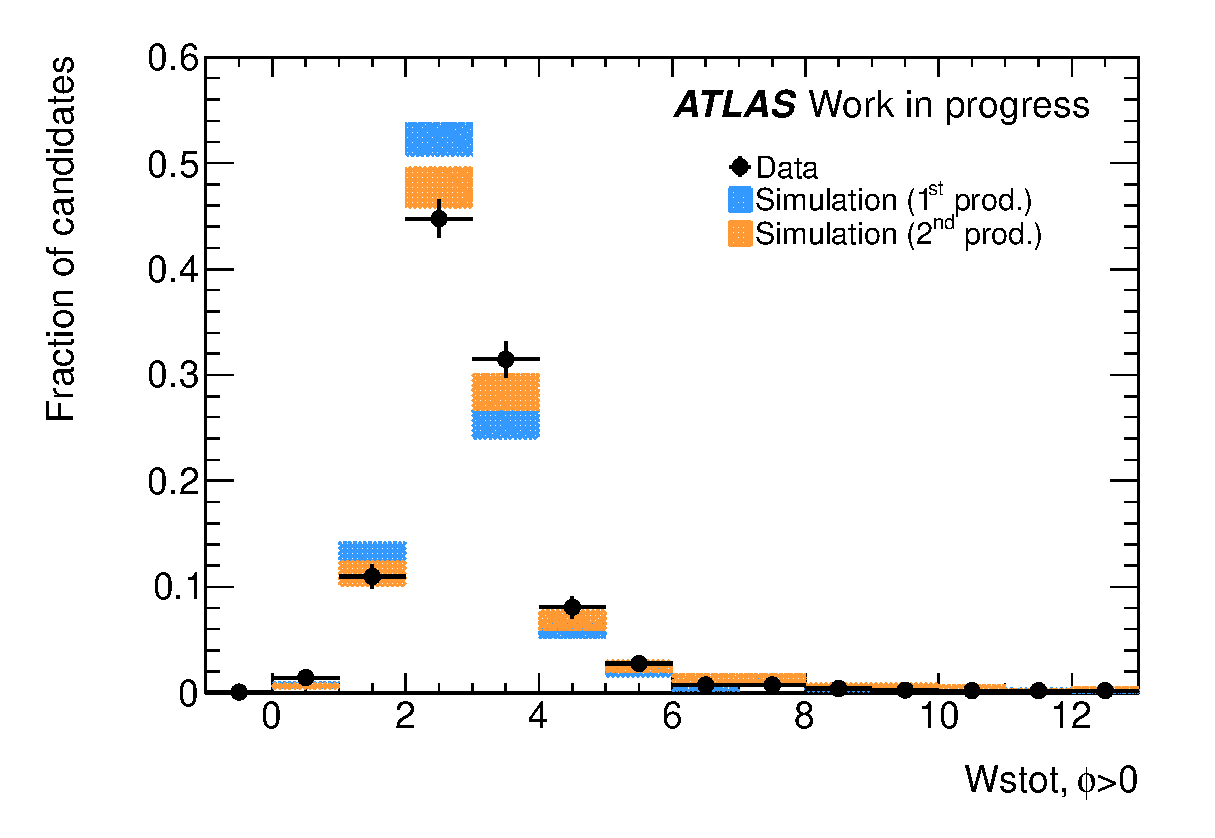
\includegraphics[height=5.25cm, keepaspectratio]{phd_cosmics/wstotUp}
    \\
    (a) & (b)
  \end{tabular}

  \end{center}
  \caption{}
\end{figure}

\begin{figure}[!ht]
  \begin{center}

  \begin{tabular}{cc}
    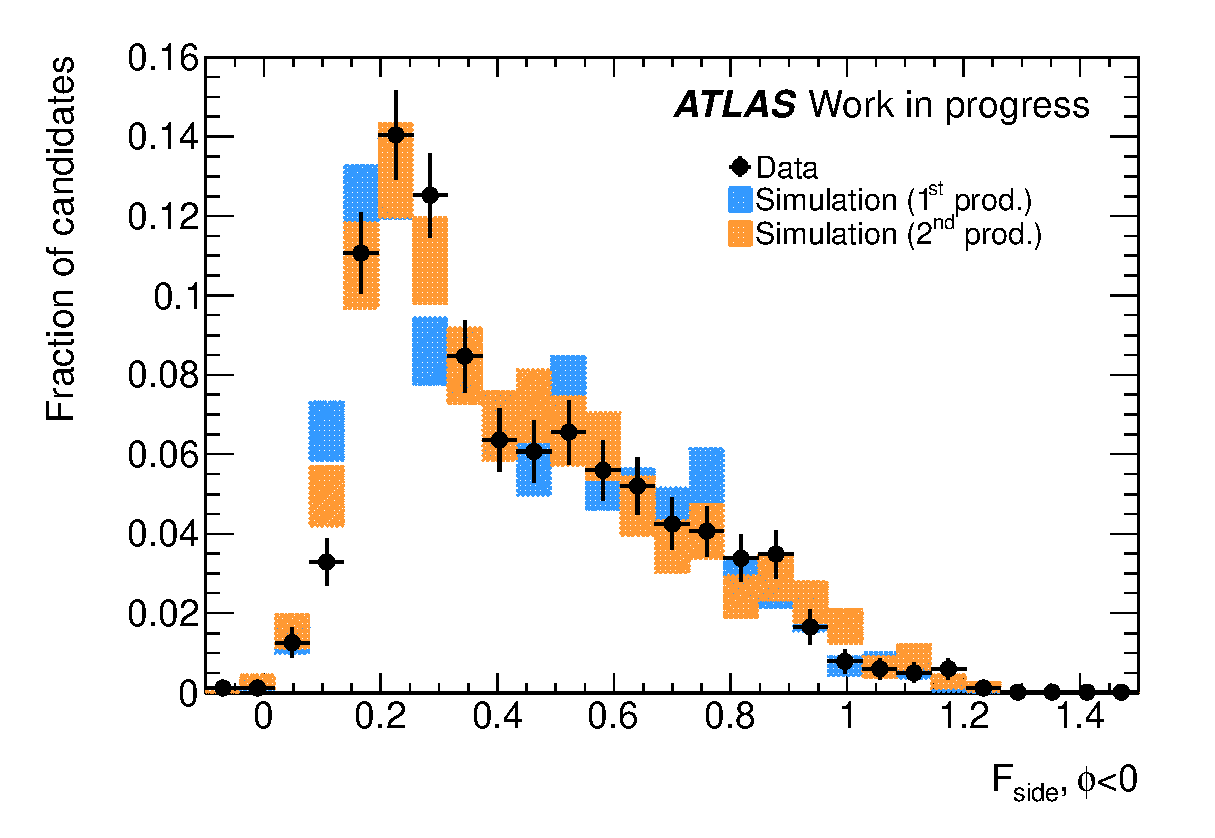
\includegraphics[height=5.25cm, keepaspectratio]{phd_cosmics/fsideDw}
    &
    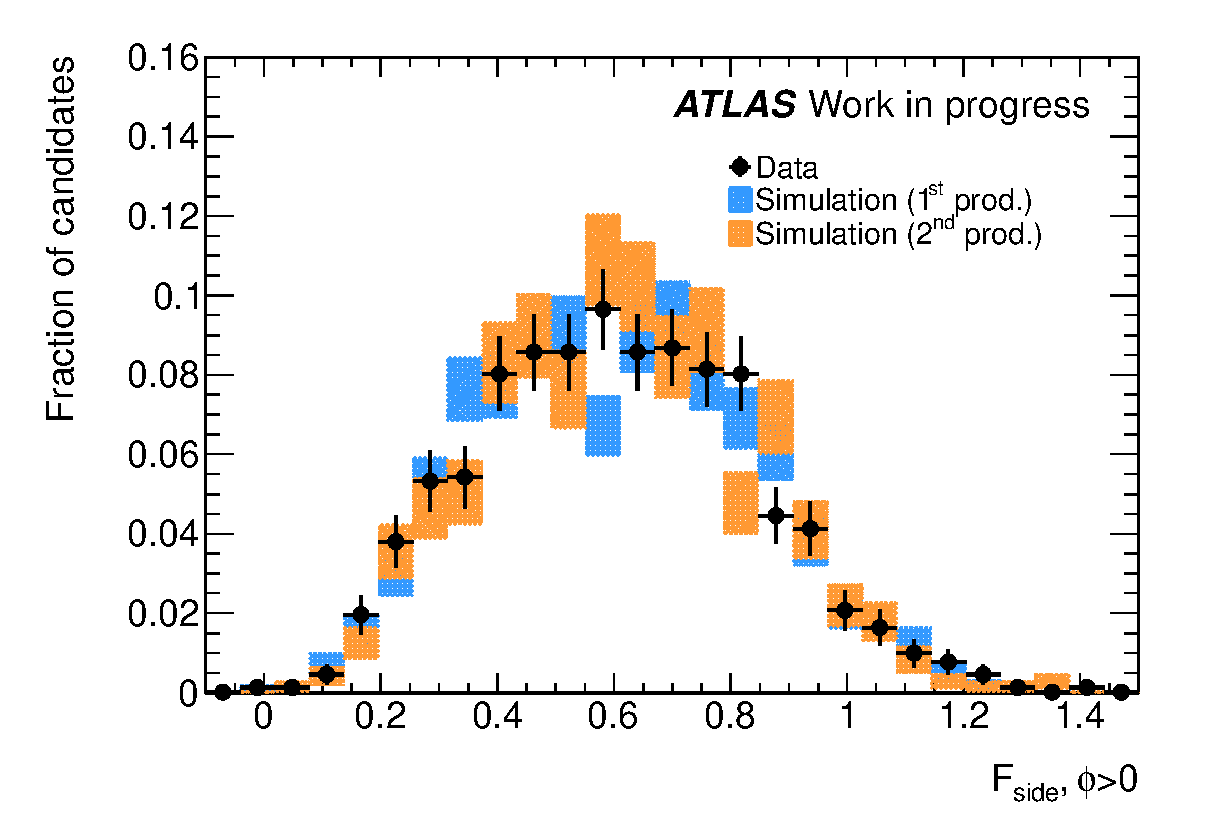
\includegraphics[height=5.25cm, keepaspectratio]{phd_cosmics/fsideUp}
    \\
    (a) & (b)
  \end{tabular}

  \end{center}
  \caption{}
\end{figure}

\begin{figure}[!ht]
  \begin{center}

  \begin{tabular}{cc}
    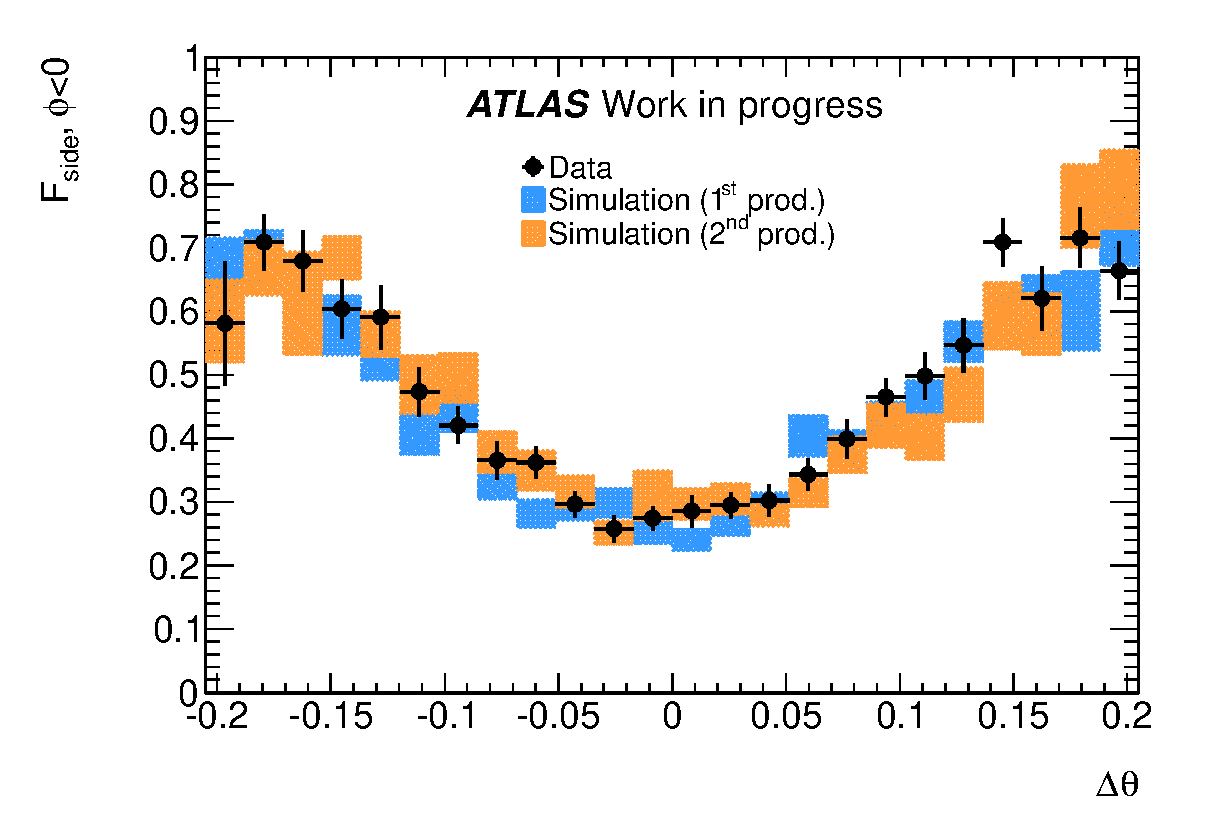
\includegraphics[height=5.25cm, keepaspectratio]{phd_cosmics/fsideDwTheta}
    &
    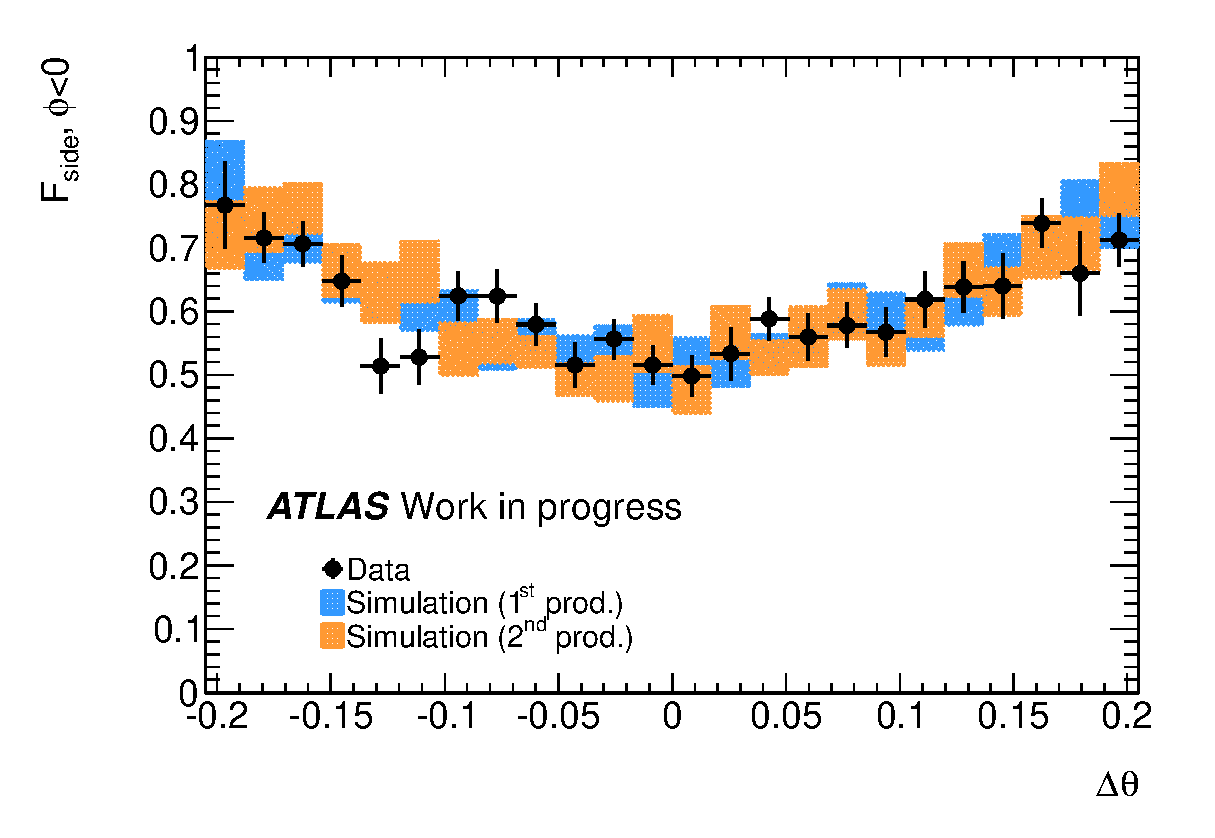
\includegraphics[height=5.25cm, keepaspectratio]{phd_cosmics/fsideUpTheta}
    \\
    (a) & (b)
  \end{tabular}

  \end{center}
  \caption{}
\end{figure}

\begin{figure}[!ht]
  \begin{center}

  \begin{tabular}{cc}
    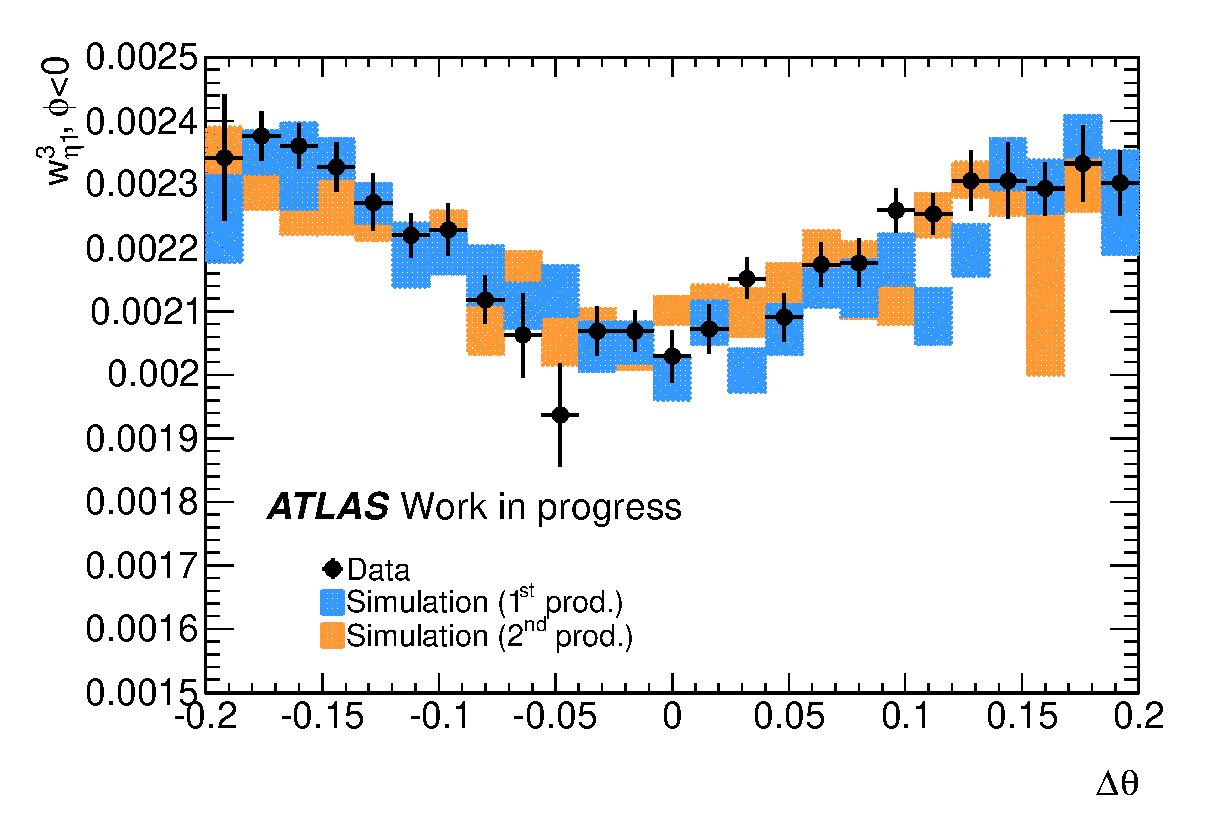
\includegraphics[height=5.25cm, keepaspectratio]{phd_cosmics/w3eta1DwTheta}
    &
    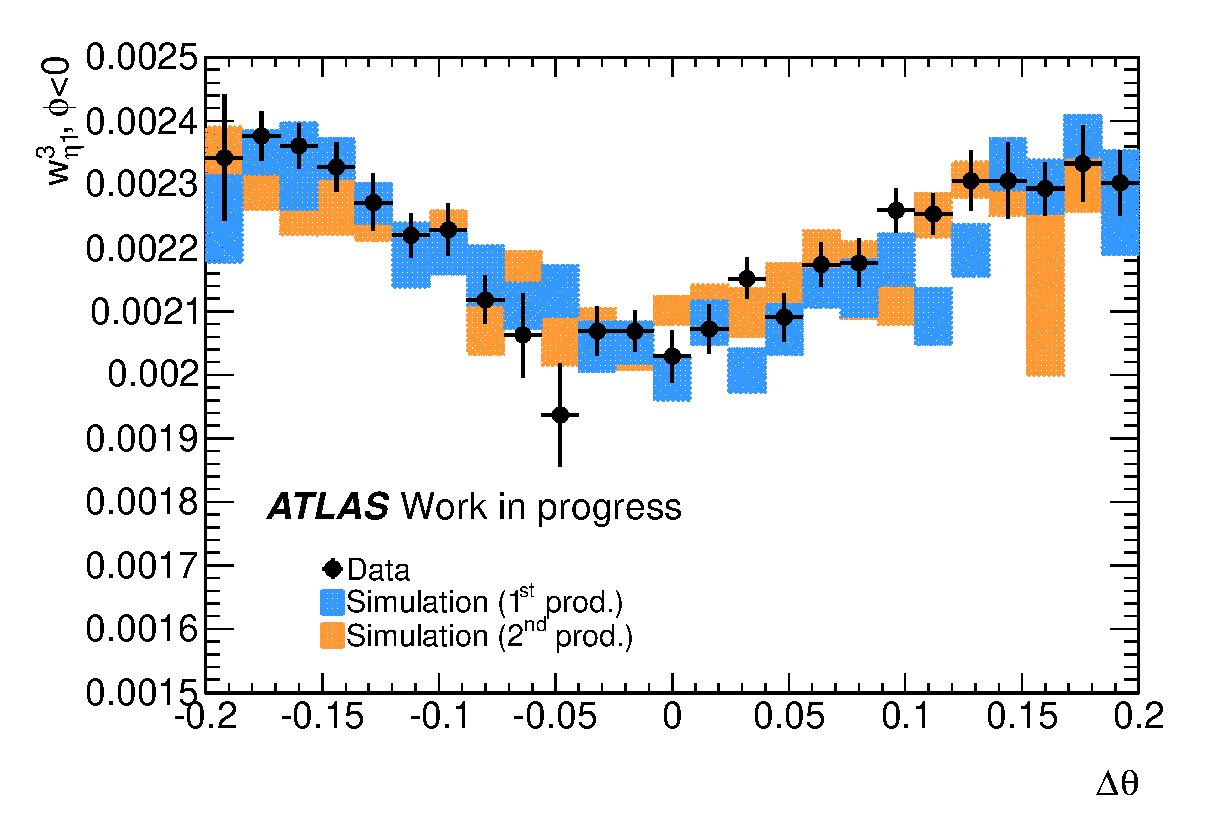
\includegraphics[height=5.25cm, keepaspectratio]{phd_cosmics/w3eta1DwTheta}
    \\
    (a) & (b)
  \end{tabular}

  \end{center}
  \caption{}
\end{figure}


